	\documentclass[10pt,oneside]{CBFT_book}
	% Algunos paquetes
	\usepackage{amssymb}
	\usepackage{amsmath}
	\usepackage{graphicx}
	\usepackage{libertine}
	\usepackage[bold-style=TeX]{unicode-math}
	\usepackage{lipsum}

	\usepackage{natbib}
	\setcitestyle{square}

	\usepackage{polyglossia}
	\setdefaultlanguage{spanish}
	



	\usepackage{CBFT.estilo} % Cargo la hoja de estilo

	% Tipografías
	% \setromanfont[Mapping=tex-text]{Linux Libertine O}
	% \setsansfont[Mapping=tex-text]{DejaVu Sans}
	% \setmonofont[Mapping=tex-text]{DejaVu Sans Mono}

	%===================================================================
	%	DOCUMENTO PROPIAMENTE DICHO
	%===================================================================

\begin{document}

% 
% =================================================================================================
\chapter{El oscilador armónico}
% =================================================================================================

Para el oscilador armónico 1D  el hamiltoniano y energía eran
\[
	H = \frac{p^2}{2m} + \frac{m\omega^2 x^2}{2} \qquad E = \hbar \omega \left( n + \frac{1}{2} \right)
\]
pero este problema puede resolverse usando un nuevo operador $\hat{a}$
\[
	\hat{a} = \sqrt{\frac{m\omega}{2\hbar}}\left( x + i\frac{p}{m\omega} \right) \qquad \text{con} \quad 
	\hat{a}^\dagger = \sqrt{\frac{m\omega}{2\hbar}}\left( x - i\frac{p}{m\omega} \right)
\]
que es suma de $\hat{x}, \hat{p}$ pero que no es hermítico. Cumple que 
\[
	[a , a^\dagger ] = 1 \qquad a a^\dagger =  \frac{H}{\hbar\omega} -1 \qquad 
	H = \hbar\omega \left( a a^\dagger + \frac{1}{2} \right),
\]
donde se define el operador número $\hat{N}\equiv a^\dagger a$ que al verificar $[\hat{N},\hat{H}]=0$ tienen 
base de 
autoestados en común $\{ \Ket{n} \}$. En efecto 
\[
	\hat{N} \Ket{n} = n\Ket{n} \qquad
	\hat{H} \Ket{n} = \hbar\omega \left( n + \frac{1}{2} \right) \Ket{n}
\]
siendo $n$ el número de cuantos de energía.
Se cumplen además 
\[
	[N,a] = [a^\dagger a,a] = - [ a, a^\dagger a ] = - \left( a^\dagger [a,a] + [a,a^\dagger]a \right) =
	-a
\]
\[
	[N,a^\dagger] = [a^\dagger a, a^\dagger ] = - [a^\dagger , a^\dagger a ] =
	- \left( a^\dagger [a^\dagger,a] + [a^\dagger,a]a^\dagger \right) = a^\dagger
\]

Queremos ver que le  hace $a^\dagger$  a un autoestado $\Ket{n}$ y luego $a$ sobre el mismo.
\[
	N a^\dagger \Ket{n} = ([N, a^\dagger] + a^\dagger N) \Ket{n} =
	a^\dagger \Ket{n} + a^\dagger n \Ket{n} 
\]
\[
	\Hat{N} (a^\dagger\Ket{n}) = (n+1)(a^\dagger\Ket{n})
\]
Entonces, como no hay degeneración y tenemos $N\Ket{n'} = n'\Ket{n'}$ entonces 
\[
	a^\dagger \Ket{n} = c_1 \Ket{n+1},
\]
y procediendo de modo idem para $a\ket{n}$ será
\[
	a \Ket{n} = c_2 \Ket{n-1}
\]
Luego,
\[
	a^\dagger \Ket{n} = c_1 \Ket{n+1} \overbrace{\longrightarrow}^{DC} 
	\Bra{n+1} c_1^* = \Bra{n} a 
\]
\[
	a \Ket{n} = c_2 \Ket{n-1} \overbrace{\longrightarrow}^{DC} \Bra{n-1} c_2^* = \Bra{n} a^\dagger
\]
y entonces 
\[
	\Braket{n|N|n} = n \Braket{n|n} = n =  \Braket{n| a^\dagger a |n} =  \Braket{n-1|c_2^* c_2|n-1} =
	|c_2|^2 \Braket{n-1|n-1}
\]
\[
	n = \Braket{n|aa^\dagger-1|n} = -1 + \Braket{n|aa^\dagger|n} = - 1 + \Braket{n+1|c_1^*c_1|n+1} =
	-1 + |c_1|^2 \Braket{n+1|n+1}
\]
siendo
\[
	|c_2| = \sqrt{n} \qquad |c_1| = \sqrt{n+1} 
\]
\[
	\hat{a}^\dagger \Ket{n} = \sqrt{n+1} \Ket{n+1} \qquad  \hat{a}\Ket{n} = \sqrt{n} \Ket{n-1} 
\]
y entonces de esta forma $\hat{a}^\dagger$ es el operador de creación de cuantos y $\hat{a}$ el de 
aniquilación.

\subsection{El estado fundamental $\Braket{0}$}

\[
	a \Ket{n}  \overbrace{\longrightarrow}^{DC} \Bra{n} a^\dagger
\]
y desde el postulado para productos internos,
\[
	(\Bra{n}a^\dagger)(a\Ket{n}) \geq 0 \quad n \Braket{n|n} \geq 0 \Rightarrow n \geq 0 
\]
entonces $n$ cabalga por los naturales.
Si hacemos 
\[
	a\Ket{n} = \sqrt{n} \Ket{n-1}, \qquad  a^2 \Ket{n} = \sqrt{n}\sqrt{n-1} \Ket{n-2} \; ...
\]
en algún momento se llega a $\Ket{n=0}$, entonces $E_0 = \hbar\omega/2$ y 
\[
	\Ket{0} \equiv \text{El fundamental}
\]
y no se puede bajar más,
\[
	\hat{a}\Ket{0} = 0.
\]

Por otra parte, con el $\hat{a}^\dagger$ se puede llegar a cualquier estado
\[
	a^\dagger \Ket{0} = \sqrt{1} \Ket{1}, \qquad  a^{\dagger 2} \Ket{0} = \sqrt{1}\sqrt{2} \Ket{2} = 
	\sqrt{1}\sqrt{2}\sqrt{3} \Ket{3}
\]
\[
	\frac{{(a^{\dagger})}^n}{\sqrt{n}!} \Ket{0} = \Ket{n}
\]

Las matrices de $\hat{a},\hat{a}^\dagger$ sólo tienen una diagonal corrida de elementoss 
\[
	\Braket{n'|a|n} = \sqrt{n} \Braket{n'|n-1} = \sqrt{n} \delta_{n',n-1}
\]
\[
	\Braket{n'|a^\dagger|n} =  \sqrt{n-1} \Braket{n'|n+1} = \sqrt{n-1} \delta_{n',n+1}
\]

También puede verse que 
\[
	\Braket{n|x|n}= 0 \qquad \Braket{n|p|n}= 0
\]
y por ello 
\[
	\Braket{(\Delta x)^2}_{\Ket{0}} \Braket{(\Delta p)^2}_{\Ket{0}} = \frac{\hbar^2}{4} 
\]
el estado fundamental es el de incerteza mínima.

\subsection{Función de onda}

Siendo $\Psi_n(x') = \Braket{x'|n}$ quiero evaluar $\Psi_0(x') = \Braket{x'|0}$ y ver que como 
\[
	\Braket{x'|a|0}= 0 
\]
tengo 
\[
	0 = \sqrt{ \frac{m\omega}{2\hbar} } \Braket{x'|x+\frac{ip}{m\omega}|0} =
	\sqrt{ \frac{m\omega}{2\hbar} } \left[ x'\Braket{x'|0} + \frac{i}{m\omega}\Braket{x'|p|0} \right]
\]
\[
	x' \Braket{x'|0} + \frac{i}{m\omega} (-i\hbar) \dpar{}{x} \Braket{x'|0} = 0
\]
entonces 
\[
	x' \Braket{x'|0} = - \frac{\hbar}{m\omega} \dpar{}{x'}\Braket{x'|0} 
\]
\[
	- \int \frac{m\omega}{\hbar} x' dx' = \int \frac{d \Braket{x'|0}}{\Braket{x'|0}} \Rightarrow 
	\Braket{x'|0} = \kappa \euler^{-m\omega x^{'2}/(2\hbar)}
\]
y entonces 
\[
	1 = \int_{-\infty}^{\infty} \Braket{0|x'}\Braket{x'|0} dx' = 
	\int_{-\infty}^{\infty} |\kappa|^2 \euler^{-m\omega x^{'2}/\hbar} dx' =
	|\kappa|^2 \sqrt{\frac{\pi\hbar}{m\omega}} 
\]
\[
	|\kappa| = \left( \frac{m\omega}{\pi\hbar} \right)^{1/2} = \frac{1}{(\pi x_0^2)^{1/4}}
\]
donde usamos el conocido resultado $\int_{-\infty}^\infty \exp( - a x^2) dx = \sqrt{\pi/a}$, llegamos al 
llamado pack 
gaussiano.
\[
	\Braket{x'|0} = \frac{1}{(\pi x_0^2)^{1/4}} \euler^{-\frac{1}{2}\left( x'/x_0 \right)^2}
\]
El estado fundamental tiene incerteza mínima y debe corresponder a un paquete gaussiano.

Notemos que $\hat{a}^\dagger$ crea sobre ket y aniquila sobre bra, mientras que $\hat{a}$ aniquila sobre ket 
y 
crea 
sobre bra,
\[
	a^\dagger \Ket{n} = \sqrt{n+1} \Ket{n+1} \Rightarrow \Bra{n} a = \Bra{n+1} \sqrt{n+1}
\]
\[
	a \Ket{n} = \sqrt{n} \Ket{n-1} \Rightarrow \Bra{n} a^\dagger = \Bra{n-1} \sqrt{n}
\]

\subsection{Interferencia en experimento de Young}

Consideremos la situación depicted en la figura bajo estas líneas

\begin{figure}[htb]
	\begin{center}
	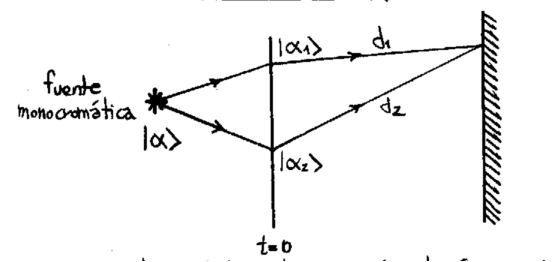
\includegraphics[width=0.6\textwidth]{images/teo2_6.pdf}	 
	\end{center}
	\caption{}
\end{figure} 

Uso $\hat{H}$ de partículas libres.
\[
	\frac{1}{2} \Ket{\alpha} = \Ket{\alpha_1} = \Ket{\alpha_2}
\]
para $t>0$ se tiene 
\[
	\Ket{\tilde{\alpha_1}} = \euler^{ -i H t /\hbar } \Ket{\alpha_1} =
		\euler^{ -i E_\alpha t /\hbar } \Ket{\alpha_1}	
\]
\[
	\Ket{\tilde{\alpha_2}} = \euler^{ -i E_\alpha t /\hbar } \Ket{\alpha_2}	
\]

En la pantalla debe verse la interferencia de los dos estados solapados.
\[
	\Ket{\tilde{\alpha}} = \Ket{\tilde{\alpha_1}} + \Ket{\tilde{\alpha_2}} =
		\euler^{ -i E_\alpha \frac{d_1}{v} /\hbar } \Ket{\alpha_1} +
		\euler^{ -i E_\alpha \frac{d_2}{v} /\hbar } \Ket{\alpha_2}	
\]
\[
	\Ket{\tilde{\alpha}} = \frac{1}{2} \euler^{ -i E_\alpha \frac{d_1}{v} /\hbar } 
		| 1 + \euler^{ -i E_\alpha \frac{d_2-d_1}{v} /\hbar } | \Ket{\alpha_1}
\]
y si definimos
\[
	\beta=E_\alpha \frac{d_2-d_1}{v} /\hbar,
\]
resulta entonces
\[
	\Braket{\tilde{\alpha}|\tilde{\alpha}} = \frac{1}{4}| 1 +  \euler^{ -i E_\alpha \frac{d_2-d_1}{v} 
/\hbar } |^2 =
		\frac{1}{4}( (1+\cos\beta)^2 + \sin^2\beta ) =
			\frac{1}{2} + \frac{1}{2}\cos\left( \beta \right).
\]


Al partir el estado $\Ket{\alpha_1} $ y volver a unirlo en $\Ket{\alpha_1} + \Ket{\alpha_2}$ vemos una 
intensidad que 
dependa de la diferencia de camino.

\subsection{Cambio de cero del potencial}

En mecánica clásica la física de un problema no se ve afectada por un cambio de gauge.
Si movemos el cero de potencial, la situación física es la misma.
Veamos qué sucede en mecánica cuántica.
\[
	\Ket{\alpha,t,t_0} = \euler^{ -i (p^2/2m + V(x))(t-t_0)/\hbar} \Ket{\alpha,t_0}
\]
\[
	\Ket{\tilde{\alpha},t,t_0} = \euler^{ -i (p^2/2m + V(x) + V_0)(t-t_0)/\hbar} \Ket{\alpha,t_0}
\]
\[
	\Ket{\tilde{\alpha},t,t_0} = \euler^{ -i V_0(t-t_0)/2 }\Ket{\alpha,t,t_0}
\]
y entonces vemos que $\Ket{\tilde{\alpha},t}$ y $\Ket{\alpha,t}$ difieren en una fase, de manera que los 
valores de 
expectación no cambian (con $V_0$ constante).

\begin{figure}[htb]
	\begin{center}
	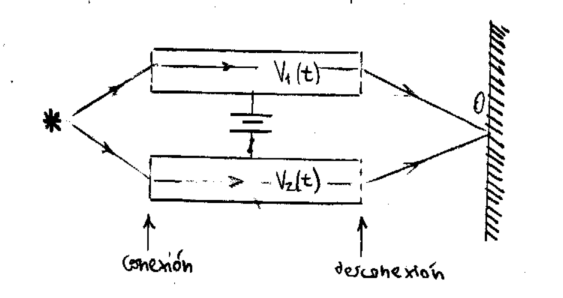
\includegraphics[width=0.6\textwidth]{images/teo2_7.pdf}	 
	\end{center}
	\caption{}
\end{figure} 

Este es un experimento ideal (pensado). Dentro de los cilindros hay campo nulo. Se varia el $V$ abriendo y 
cerrando la 
llave a la entrada y a la salida.
Se cambia la fase de las partículas inferiores respecto de las superiores, entonces habrá interferencia en 
$O$.

Clásicamente no hay variación,
\[
	\Delta \text{fase} = -\frac{i}{\hbar}\euler \int _{t_1}^{t_2} V_1(t) - V_2(t) dt = 
	-\frac{i}{\hbar}\euler \Delta V
\]

Lo que realmente cuenta es la diferencia de potencial $\Delta V$, la cual sí tiene sentido físico porque es 
independiente de la medida y porque pueden escribirse los campos en función de aquella.
\[
	E = - \Nabla\phi - \frac{1}{c}\dpar{\vb{A}}{t}
\]
\[
	H = \frac{1}{2m} \left( \vb{p} - \frac{\euler\vb{A}}{c}\right)^2 + \euler\phi 
\]
\[
	\dtot{H}{t} = \frac{1}{i\hbar}[x_i,H] = \frac{p_i  \euler A_i}{m}
\]

% =================================================================================================
\section{El propagador}
% =================================================================================================

Físicamente representa la proababilidad de transición entre autoestados por el paso del tiempo,
$ \Ket{x'}_{t_0} \longrightarrow \Ket{x''}_t$
\[
	\Braket{x''|\euler^{-iH(t-t_0)/\hbar}|x'} \equiv K(x',t; x, t_0)
\]
\[
	\Braket{x''| \alpha,t_0,t} = \Braket{x''|\euler^{-iH(t-t_0)/\hbar}|\alpha,t_0} 
\]
\[
	\Braket{x''| \alpha,t_0,t} = \int dx' \Braket{x''|\euler^{-iH(t-t_0)/\hbar}|x'}\Braket{x'|\alpha,t_0} 
\]
\[
	\Psi_{\alpha}(x'',t) = \int dx' K(x'',t; x',t) \Psi_{\alpha}(x',t)
\]

Podemos pensar que el propagador lleva la función de onda desde $t_0$ a $t$. Se puede escribir:
\[
	K(x',t; x, t_0) = \sum_{a'} \Braket{x''|a'} \Braket{a'|x'} \euler^{-iE_a(t-t_0)/\hbar}
\]
y metemos un observable $\hat{A}$ donde $[A,H]=0$ y $A\Ket{a'}=a\Ket{a'}$.

El propagador depende del potencial, pero no de la función de onda inicial. Se debe cumplir que:
\[
	\lim_{t\to t_0} K(x',t; x, t_0) = \delta^3(x''-x')
\]
\[
	K(x'',t; x, t_0) = \Braket{x''|\euler^{-iH(t-t_0)/\hbar}|a'} \Braket{a'|x'} =
		\sum_{a'} \Psi_{\Ket{a'}}(x'',t)\Braket{a'|x'}
\]
\[
	K(x'',t; x, t_0) = \sum_{a'} c_{a'}(x')\Psi_{\Ket{a'}}(x'',t)
\]
y entonces el propagador es una función de Green que satisface 
\[
	\left( -\frac{\hbar^2}{2m}\nabla^2 +V(x'') - i\hbar\dpar{}{t} \right)K(x',t; x, t_0) =
		- i\hbar \delta^3(x''-x') \delta(t-t_0)
\]
con $K(x'',t;x',t_0)=0 $ si $t<0$ que es la condición de contorno.

\subsection{El propagador de la partícula libre}

\[
	K(x'',t; x, t_0) = \int dp' \Braket{x''|\euler^{-ip^2(t-t_0)/2m\hbar}|p'} \Braket{p'|x'} 
\]
\[
	= \int dp' \euler^{-ip'^{2}(t-t_0)/2m\hbar} \Braket{x''|p'} \Braket{p'|x'} =
	\frac{1}{2\pi\hbar} \int dp' \euler^{-ip'^{2}(t-t_0)/2m\hbar} \euler^{-ip'(x'-x'')/\hbar}
\]
y entonces el propagador de una partícula libre es
\[
	K(x'',t; x, t_0) = \sqrt{ \frac{m}{2\pi\hbar(t-t_0)} } \euler^{i\frac{m(x''-x')^2}{2\hbar(t-t_0)}}
\]

También se puede escribir el propagador en la representación de Heisenberg,
\[
	\Braket{x''|\euler^{-iH(t-t_0)/\hbar}|x'} = \Bra{x''}\euler^{-iHt/\hbar} \euler^{iHt_0/\hbar}\Ket{x'}=
		\Braket{x'',t|x',t_0}
\]
\[
	K(x'',t;x',t_0) = \Braket{x'',t | x',t_0}.
\]

El propagador cumple con la propiedad de composición (como el $U(t,t_0)$), es decir:
\[
	K(x'',t; x, t_0) = K(x'',t; x, t_1)K(x'',t_1; x, t_0) \qquad t>t_1>t_0
\]

% =================================================================================================
\section{Integrales de camino de Feynmann}
% =================================================================================================

Consideramos una partícula yendo de $(x_1,t_1)$ a $(x_N,t_N)$. Dividimos el tiempo 
\[
	a
\]
y queremos ver la amplitud de transición desde el estado 1 al $N$.

\begin{figure}[htb]
	\begin{center}
	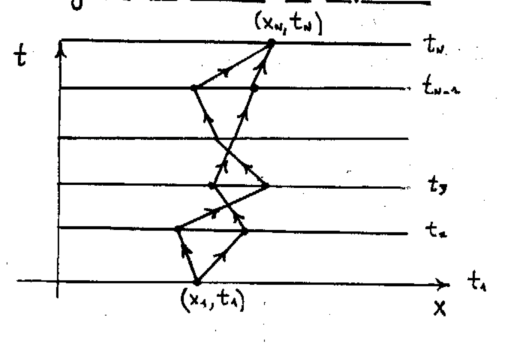
\includegraphics[width=0.6\textwidth]{images/teo2_8.pdf}	 
	\end{center}
	\caption{}
\end{figure} 

\[
	a
\]

Se puede pensar como que estamos sumando sobre todos los posibles caminos entre $(x_1,t_1)$ y $(x_N,t_N)$ 
fijos. En mecánica clásica teníamos un solo camino, el que minimizaba la acción $S$
\[
	\delta \int_{t_1}^{t_2} \Lag dt = \delta S = 0
\]
pero en cambio en mecánica cuántica todos los caminos aportan. En un libro de Dirac, Feymann lee 
\[
	a
\]
Definiremos
\[
	\equiv 
\]
Luego para considerar la suma sobre todos los segmentillos a lo largo de un camino tendremos
\[
	\prod_{n=2}^N \euler^{i/\hbar S(n,n-1)} =
\]
y hay que considerar TODOS los posibles caminos 
\[
	\propto \sum_{caminos} \euler^{i/\hbar S(N,1)} 
\]
cuando $\hbar \to 0$ las trayectorias contribuyen con una cantidad que oscila loca y violentamente. Tienden a 
la cancelación para caminos aledaños. Por el $\hbar \sim 0$ la fase es grande y entonces se cancelan.
Esto no ocurre cerca del camino (real) que cumple 
\[
	\delta S(N,1) = 0
\]
Para trayectorias cercanas la $\Delta fase$ no es grande y hay interferencia constructiva.
Para un $\delta t$ infinitesimal es 
\[
	a
\]
\[
	b
\]

\begin{figure}[htb]
	\begin{center}
	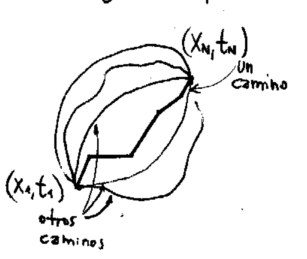
\includegraphics[width=0.6\textwidth]{images/teo2_9.pdf}
	\end{center}
	\caption{}
\end{figure} 

Consideremos, por ejemplo, una partícula libre, entonces $V=0$ de modo que resolviendo 
\[
	a
\]
Esto no es otra cosa que el propagador de una partícula libre. Para un $\Delta t$ finito será 
\[
	+
\]
\[
	=
\]
siendo esta última la integral de camino de Feynmann.

En base a éstas Feynamn desarrolla una formulación equivalente de la mecánica cuántica que utiliza los 
conceptos de:
\begin{enumerate}
 \item Superposición
 \item Composición de la transición
 \item Límite clásico con $\hbar \to 0$
\end{enumerate}

Estas integrales contienen toda la información del sistema cuántico, aunque no sea sencillo extraerla.

Consideremos un propagador de $(x',0) \to (x',t)$
\[
	G(t) =
\]
\[
	G(t) =
\]
y tomando Laplace-Fourier 
\[
	\tilde{G}(t)
\]

La expresión 
\[
	\equiv Integral de camino de Feynmann
\]
satisface la ecuación de Schrödinger y es una alternativa a la formulación de la cuántica usual.


% \bibliographystyle{CBFT-apa-good}	% (uses file "apa-good.bst")
% \bibliography{CBFT.Referencias} % La base de datos bibliográfica

\end{document}
